\begin{appendices}

\section{Likelihood estimation by importance sampling}
\label{app:NLLestimateImportSampling}

The marginal likelihood $p(x)$ is estimated using importance sampling by generating $S$ samples from some sampling distribution $p_\textrm{samp}(z|x)$ and using the following estimation:
\begin{equation}
p(x) = \E_{z \sim p_\textrm{samp}} \left[\frac{p(x|z) \cdot \pi(z)}{p_\textrm{samp}(z|x)} \right] \approx \frac{1}{S} \sum_{s=1}^S \frac{p(x|z_s) \cdot \pi(z_s)}{p_\textrm{samp}(z_s|x)} \textrm{ for } z_s \sim p_\textrm{samp}
\end{equation}
For this estimation to be efficient it is important that the sampling distribution tightly covers the true posterior $p(z|x)$. To achieve this the sampling distribution, a multivariate Gaussian, was centred on an estimate of the mean of the true posterior, which was obtained by sampling five times from the posterior approximation, i.e.\ the HMC-enhanced encoder. For the covariance of the sampling distribution the covariance matrix of the initial encoder $q_0(z|x)$ was used.

This returned low variance estimates of the marginal likelihood with little dependence on the number of samples $S$ for $S > 2000$.

\section{Visualizations of latent space}

\begin{figure}[hb]
\centering
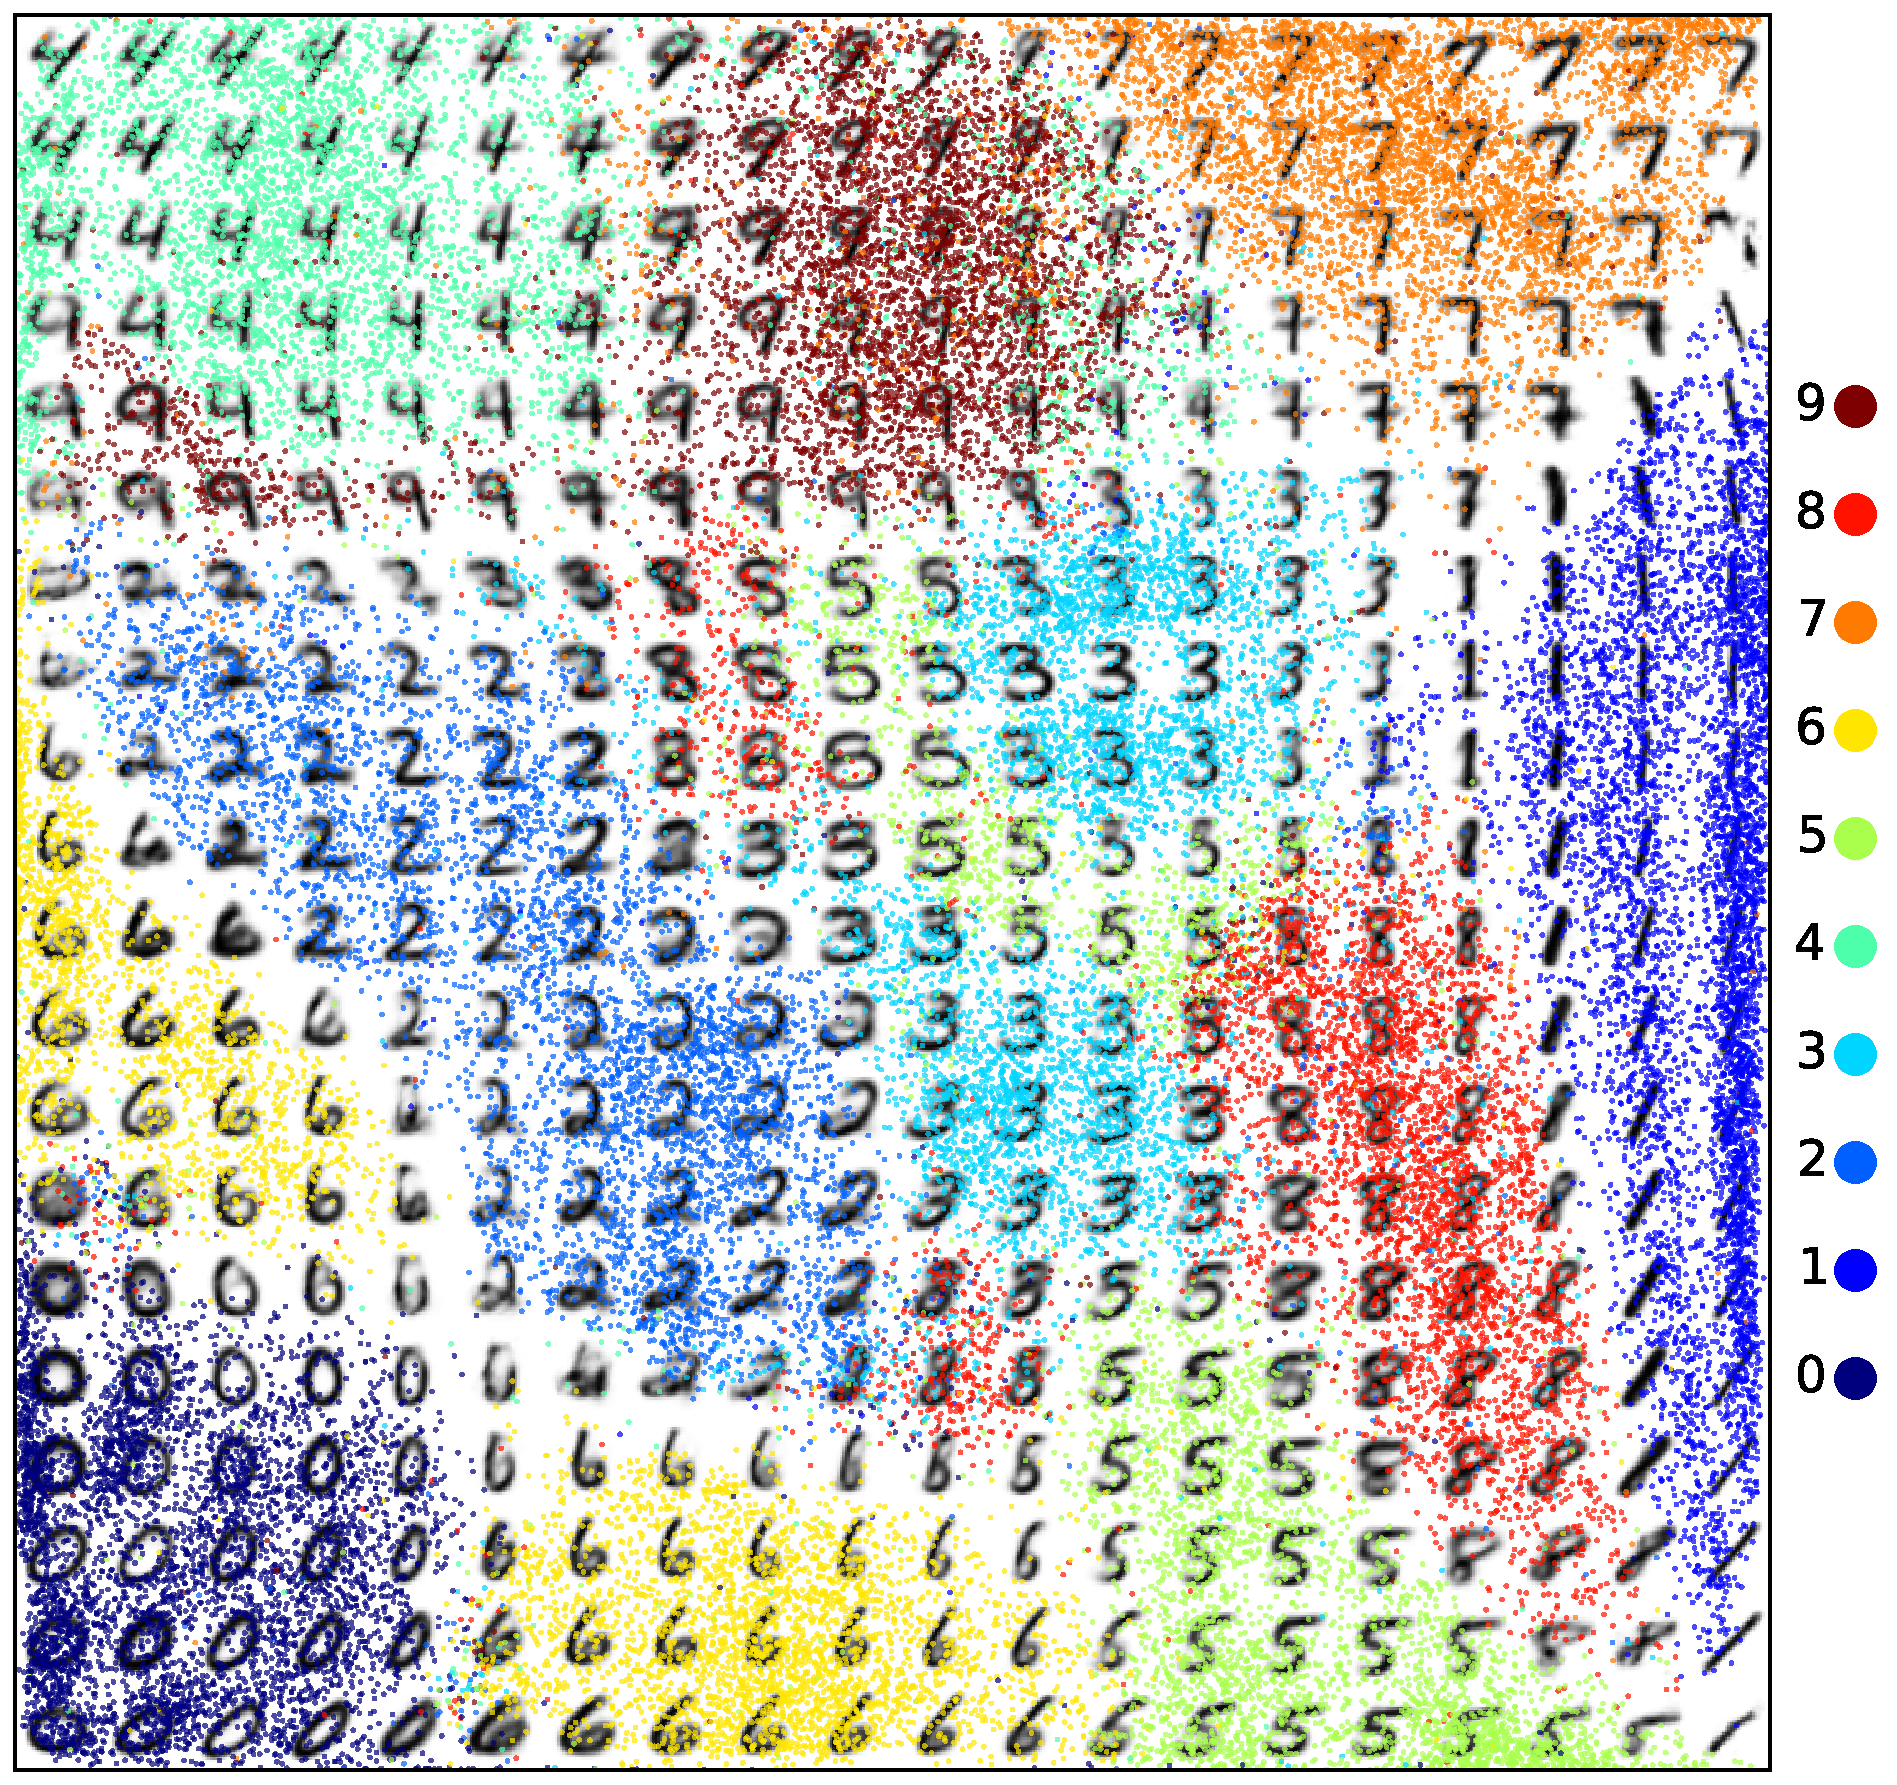
\includegraphics[width=\columnwidth]{figures/learned_representation_train_points_small.pdf}
\caption{Clever caption}
\label{fig:2d_latent_visualization}
\end{figure}

%TODO
In figure~\ref{fig:EnergySurfaceMNIST} the energy surface for a digit from the MNIST dataset (described below)

\begin{figure}
\centering
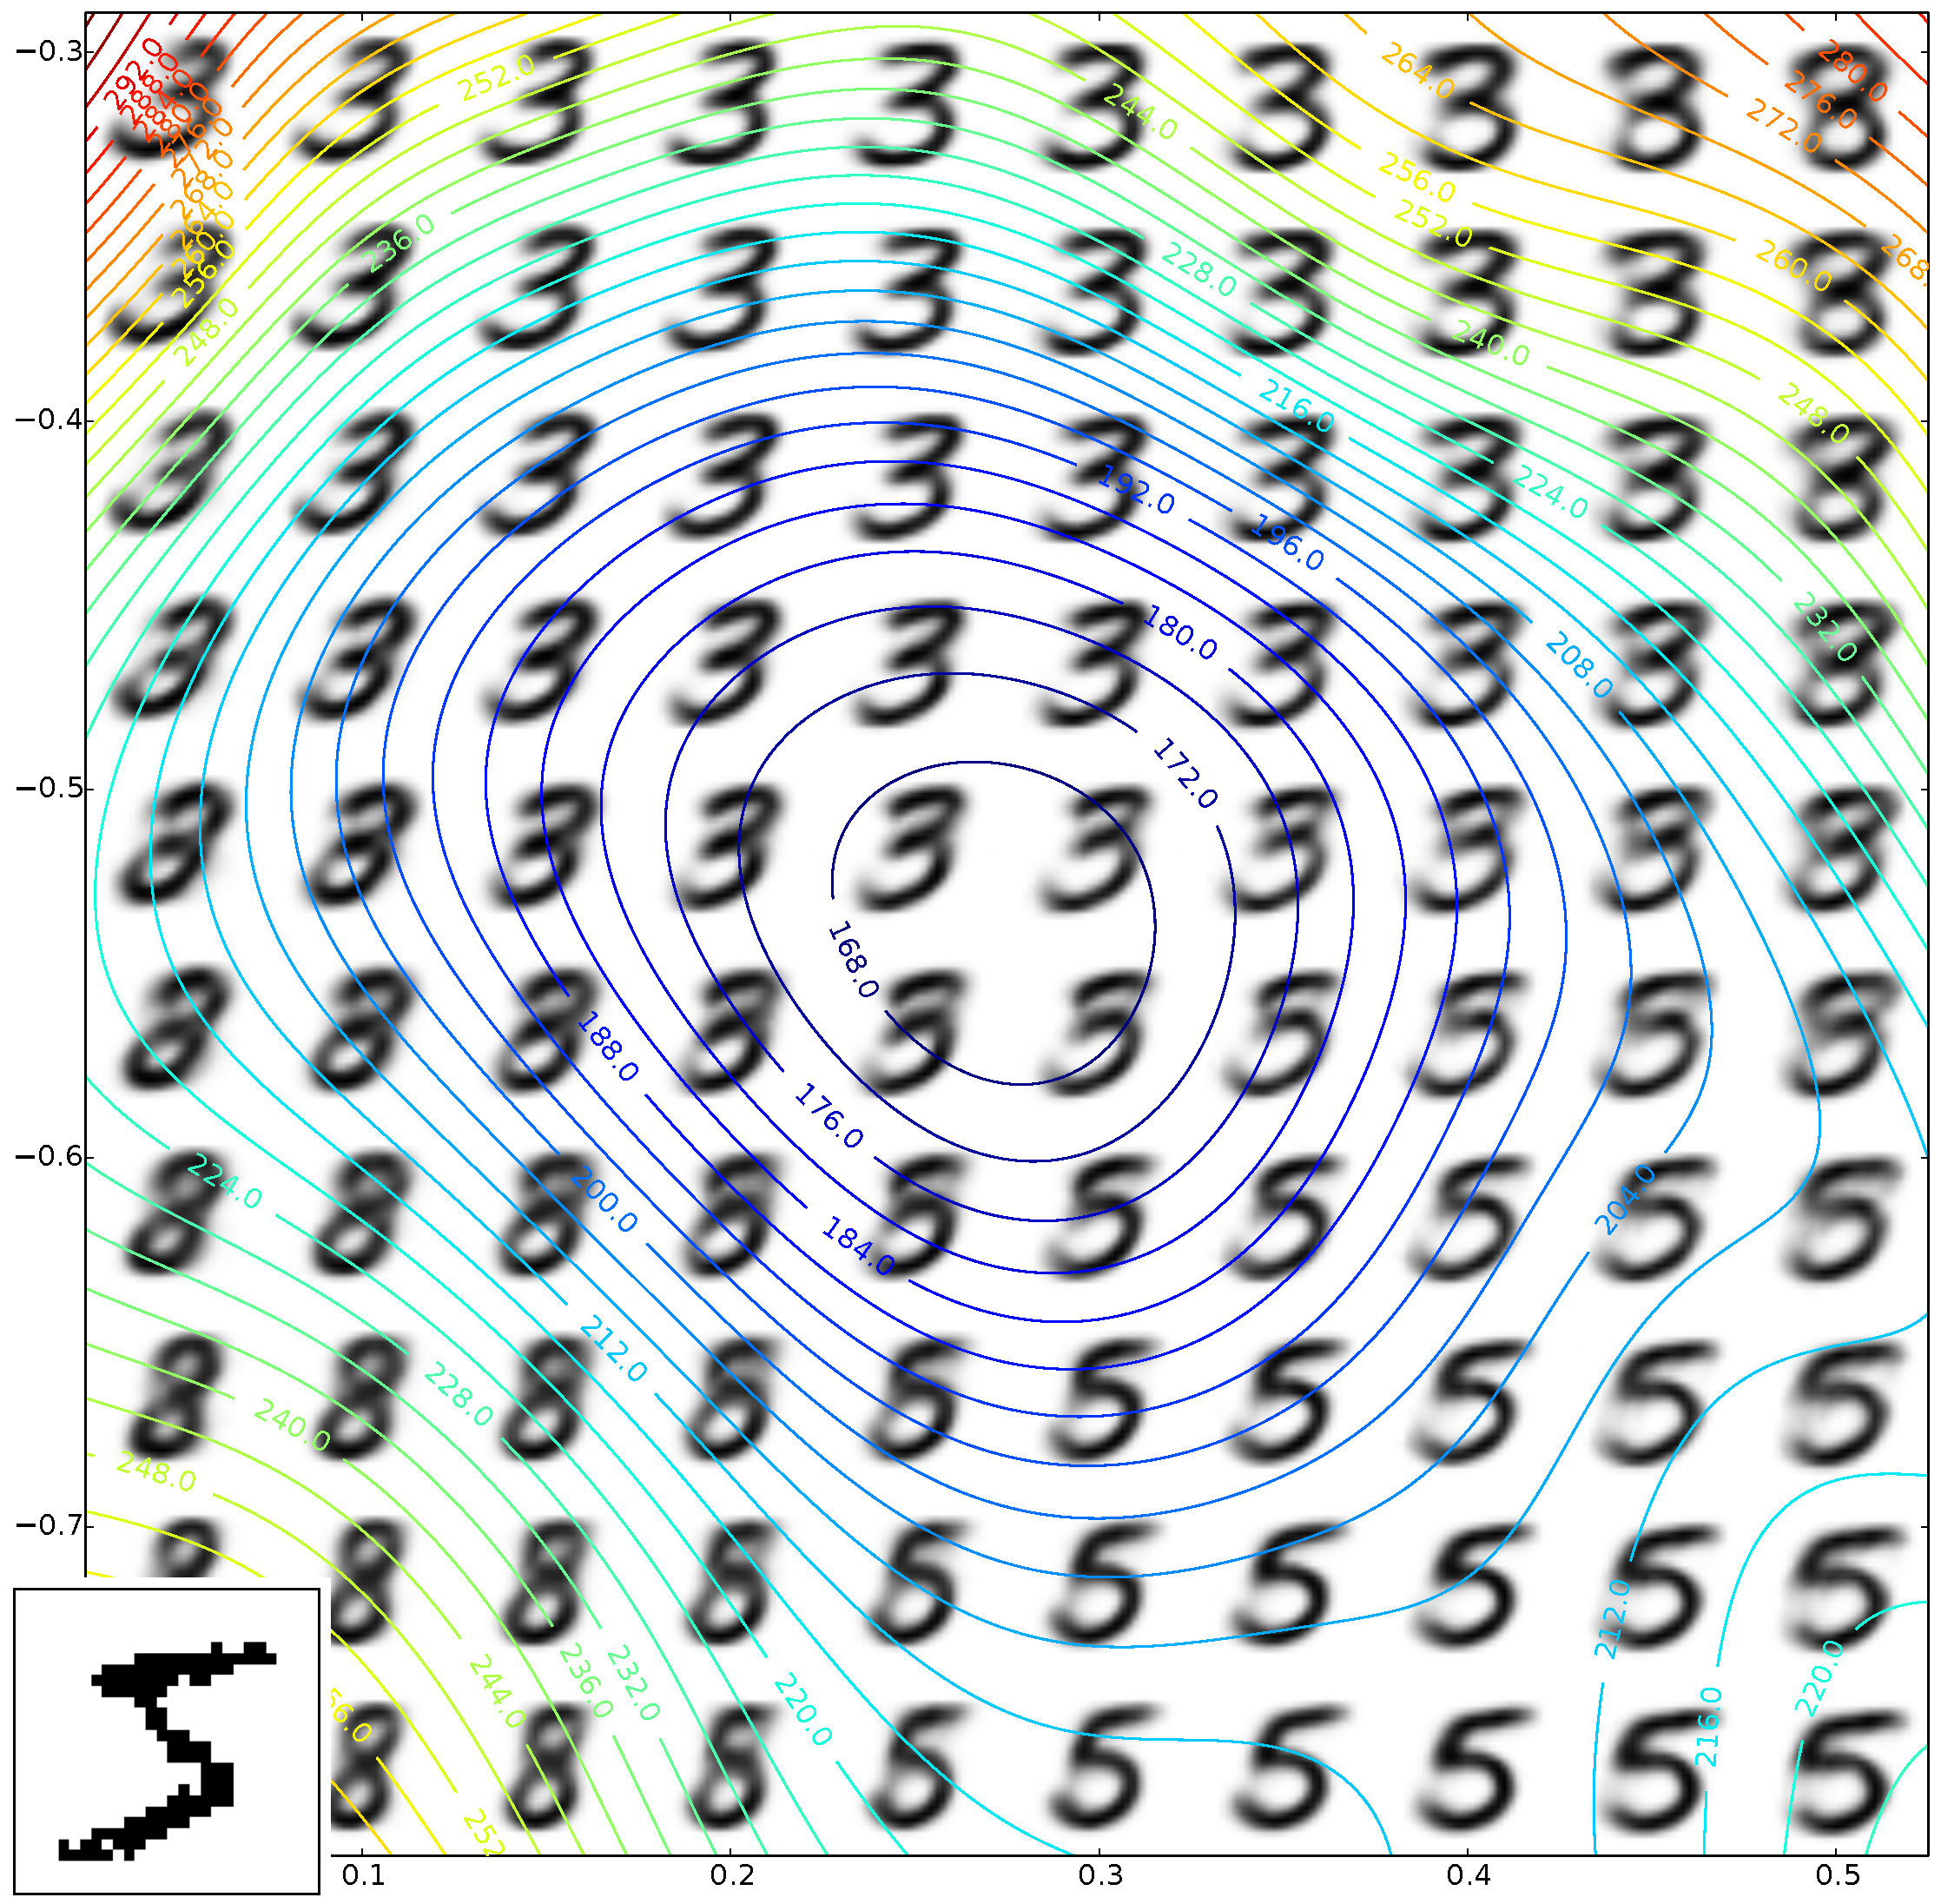
\includegraphics[width=\columnwidth]{figures/vae_pot_energy_example.pdf}
\caption{Energy surface for MNIST data. Inset show the corresponding observed digit from the MNIST dataset (see~\ref{sec:Dataset})}.
\label{fig:EnergySurfaceMNIST}
\end{figure}


\end{appendices}